\documentclass[12pt,a4paper]{article}

% ── Packages ──
\usepackage{style}

\pagestyle{fancy}
\fancyhf{}
\rhead{Benchmarking Numerical ERI Methods}
\lhead{}
\rfoot{Page \thepage}

\hypersetup{
    colorlinks=true,
    linkcolor=black,
    citecolor=black,
    urlcolor=blue
}

% ── Code listing style ──
\definecolor{codebg}{rgb}{0.97,0.97,0.97}
\definecolor{codegreen}{rgb}{0.0,0.5,0.0}
\definecolor{codepurple}{rgb}{0.58,0,0.82}

\lstset{
    language=Python,
    backgroundcolor=\color{codebg},
    basicstyle=\ttfamily\footnotesize,
    keywordstyle=\color{blue}\bfseries,
    stringstyle=\color{codepurple},
    commentstyle=\color{codegreen}\itshape,
    numbers=left,
    numberstyle=\tiny\color{gray},
    stepnumber=1,
    numbersep=6pt,
    frame=single,
    breaklines=true,
    captionpos=b,
    tabsize=4,
    showstringspaces=false,
}

% ── Title ──
\title{
    \vspace{-1cm}
    \textbf{Benchmarking Numerical Methods for Electron Repulsion Integrals: \\[4pt]
    From Direct Summation to Poisson--NUFFT Solvers}
}
\author{
    Mohammad Ahmad: 2074000

    Supervisor: Dr Johannes Margraf
}
\date{\today}

\begin{document}

\maketitle
\thispagestyle{empty}

\begin{abstract}
Electron repulsion integrals (ERIs) constitute the primary computational bottleneck in quantum chemistry simulations, scaling as $\mathcal{O}(N^4)$ in conventional analytical approaches. This report presents a systematic benchmark of seven numerical methods for computing ERIs, ranging from brute-force direct summation in real space through uniform Fast Fourier Transforms (FFT) to Non-Uniform Fast Fourier Transform (NUFFT) techniques and a two-step Poisson--NUFFT solver. We evaluate each method on the hydrogen molecule H$_2$ using the \texttt{def2-svp} basis set, measuring absolute error against the analytical PySCF reference, wall-clock time, and peak memory consumption as the grid resolution parameter $N$ increases. Our results demonstrate that the Poisson two-step method with a spherical $k$-space grid achieves the fastest convergence, reaching errors below $10^{-3}$ at moderate grid sizes, while maintaining competitive computational cost. We discuss the mathematical foundations of each approach, analyse convergence behaviour, and suggest directions for future work including extension to multi-centre integrals and GPU acceleration.
\end{abstract}

\newpage
\tableofcontents
\newpage

%==========================================================================
\section{Introduction}
\label{sec:intro}
%==========================================================================

Many advances in materials science, battery technology, semiconductor design, and superconductivity owe their progress to quantum chemistry simulations. At their core, these simulations seek approximate solutions to the many-body Schr\"{o}dinger equation:
\begin{equation}
    \hat{H}\,\Psi(\mathbf{r}_1, \ldots, \mathbf{r}_n) = E\,\Psi(\mathbf{r}_1, \ldots, \mathbf{r}_n),
    \label{eq:schrodinger}
\end{equation}
where $\hat{H}$ is the molecular Hamiltonian and $\Psi$ is the many-electron wavefunction. Under the Born--Oppenheimer approximation, the nuclei are treated as stationary point charges and the electronic Hamiltonian becomes:
\begin{equation}
    \hat{H}_{\text{elec}} = -\frac{1}{2}\sum_i \nabla_i^2
    - \sum_{i,A}\frac{Z_A}{|\mathbf{r}_i - \mathbf{R}_A|}
    + \sum_{i<j}\frac{1}{|\mathbf{r}_i - \mathbf{r}_j|},
    \label{eq:helec}
\end{equation}
where the three terms represent the kinetic energy, nuclear--electron attraction, and electron--electron repulsion respectively. The final term is the most computationally demanding.

To discretise the problem, the molecular orbitals are expanded in a basis of $K$ atom-centred functions $\{\chi_\mu\}$:
\begin{equation}
    \phi_i(\mathbf{r}) = \sum_{\mu=1}^{K} C_{\mu i}\,\chi_\mu(\mathbf{r}).
    \label{eq:lcao}
\end{equation}
Gaussian-Type Orbitals (GTOs) are the standard choice because the product of two Gaussians centred at different points yields another Gaussian (the Gaussian Product Theorem), which simplifies integral evaluation:
\begin{equation}
    \chi_\mu(\mathbf{r}) = N_\mu\,(x - A_x)^{l_x}(y - A_y)^{l_y}(z - A_z)^{l_z}\,\exp\!\bigl(-\alpha_\mu |\mathbf{r} - \mathbf{A}|^2\bigr).
    \label{eq:gto}
\end{equation}

Substituting \cref{eq:lcao} into the energy expression produces four classes of molecular integrals. The overlap integrals $S_{\mu\nu}$, kinetic energy integrals $T_{\mu\nu}$, nuclear attraction integrals $V_{\mu\nu}$, and the four-centre electron repulsion integrals (ERIs):
\begin{equation}
    (\mu\nu|\lambda\sigma) = \iint \frac{\chi_\mu(\mathbf{r}_1)\chi_\nu(\mathbf{r}_1)\;\chi_\lambda(\mathbf{r}_2)\chi_\sigma(\mathbf{r}_2)}{|\mathbf{r}_1 - \mathbf{r}_2|}\,d^3r_1\,d^3r_2.
    \label{eq:eri}
\end{equation}
For a basis of size $K$, the number of unique ERIs scales as $\mathcal{O}(K^4)$, making their evaluation the dominant computational bottleneck.

A key insight is that the Coulomb kernel has a simple form in Fourier (reciprocal) space. The Fourier transform of $1/|\mathbf{r}|$ in three dimensions is:
\begin{equation}
    \mathcal{F}\!\left[\frac{1}{|\mathbf{r}|}\right](\mathbf{k}) = \frac{4\pi}{|\mathbf{k}|^2}.
    \label{eq:coulomb_ft}
\end{equation}
This transforms the six-dimensional integral in \cref{eq:eri} into a product of three-dimensional Fourier transforms, reducing it by the convolution theorem to:
\begin{equation}
    (\mu\nu|\lambda\sigma) = \frac{1}{(2\pi)^3}\int \frac{4\pi}{|\mathbf{k}|^2}\;\widetilde{f}(\mathbf{k})\;\widetilde{g}^*(\mathbf{k})\,d^3k,
    \label{eq:eri_kspace}
\end{equation}
where $\widetilde{f}(\mathbf{k})$ and $\widetilde{g}(\mathbf{k})$ are the Fourier transforms of the overlap densities $f(\mathbf{r}) = \chi_\mu(\mathbf{r})\chi_\nu(\mathbf{r})$ and $g(\mathbf{r}) = \chi_\lambda(\mathbf{r})\chi_\sigma(\mathbf{r})$.

The Coulomb potential generated by a charge distribution $\rho(\mathbf{r})$ satisfies Poisson's equation:
\begin{equation}
    \nabla^2 V(\mathbf{r}_1) = -4\pi\,\rho(\mathbf{r}_1),
    \label{eq:poisson}
\end{equation}
with the solution:
\begin{equation}
    V(\mathbf{r}_1) = \int \frac{\rho(\mathbf{r}_2)}{|\mathbf{r}_1 - \mathbf{r}_2|}\,d^3r_2.
    \label{eq:poisson_sol}
\end{equation}
Fourier-transforming \cref{eq:poisson} converts the differential equation into the algebraic relation:
\begin{equation}
    \widetilde{V}(\mathbf{k}) = \frac{4\pi}{|\mathbf{k}|^2}\,\widetilde{\rho}(\mathbf{k}),
    \label{eq:poisson_kspace}
\end{equation}
which replaces a costly real-space integration with a pointwise multiplication in $k$-space. This is the foundation of the two-step Poisson--NUFFT solver benchmarked in this study.

The standard FFT operates on uniformly spaced grids and achieves $\mathcal{O}(N\log N)$ complexity. However, molecular systems are better described by non-uniform grids that concentrate points near the nuclei. The Non-Uniform Fast Fourier Transform (NUFFT) generalises the FFT to handle arbitrary point distributions. It computes sums of the form:
\begin{equation}
    F(\mathbf{k}_j) = \sum_{m=1}^{M} c_m\,e^{-i\,\mathbf{k}_j \cdot \mathbf{x}_m},
    \label{eq:nufft}
\end{equation}
where $\{\mathbf{x}_m\}$ are non-uniform source points and $\{\mathbf{k}_j\}$ are non-uniform target points (this is the type-3 NUFFT). The algorithm achieves $\mathcal{O}(M\log M + N\log N)$ complexity via interpolation onto an auxiliary uniform grid, FFT, and deconvolution \cite{barnett2019}.

\subsection{Objectives}

The aim of this study is to benchmark seven numerical approaches for computing ERIs, categorised as follows:
\begin{enumerate}
    \item \textbf{Direct summation} on Cartesian and Becke grids in real space,
    \item \textbf{Uniform FFT} Poisson solver on a Cartesian grid,
    \item \textbf{One-step NUFFT} with Cartesian and spherical $k$-space grids,
    \item \textbf{Two-step Poisson--NUFFT} with Cartesian and spherical $k$-space grids.
\end{enumerate}
We evaluate convergence behaviour, computational cost, and memory usage, and discuss why certain methods outperform others from a mathematical perspective.


%==========================================================================
\section{Theoretical Background}
\label{sec:theory}
%==========================================================================

To evaluate integrals numerically, we replace the continuous integral with a weighted sum over grid points:
\begin{equation}
    \int f(\mathbf{r})\,d^3r \approx \sum_{i=1}^{N} w_i\,f(\mathbf{r}_i),
    \label{eq:quadrature}
\end{equation}
where the choice of points $\{\mathbf{r}_i\}$ and weights $\{w_i\}$ determines both accuracy and efficiency.

The simplest approach tiles a cubic domain $[-L, L]^3$ with $N^3$ equally spaced points. The spacing is $\Delta x = 2L/(N-1)$ and each weight is $w_i = (\Delta x)^3$. While straightforward, Cartesian grids waste points in empty regions far from the molecule and lack resolution near nuclei where the density varies rapidly. The error converges polynomially with $N$.

\label{sec:becke}

Becke's partitioning scheme \cite{becke1988} decomposes the molecular integral into atomic contributions:
\begin{equation}
    \int f(\mathbf{r})\,d^3r = \sum_A \int w_A(\mathbf{r})\,f(\mathbf{r})\,d^3r,
    \label{eq:becke_partition}
\end{equation}
where $w_A(\mathbf{r})$ is the Becke weight function centred on atom $A$, satisfying $\sum_A w_A(\mathbf{r}) = 1$. Each atomic integral is evaluated on a product grid of radial (Gauss--Legendre or Gauss--Chebyshev) and angular (Lebedev) quadrature points, mapped via a radial transform $r = R\,h(x)$ that concentrates points near the nucleus. The Becke radial transform used in this work maps:
\begin{equation}
    r = R\,\frac{1 + x}{1 - x}, \quad x \in [-1, 1],
    \label{eq:becke_rtransform}
\end{equation}
where $R$ is a scaling parameter (set to 1.5 bohr in our implementation). This naturally places more grid points in the chemically important region near the nuclei.

In reciprocal space, we construct a spherical grid using a product of Gauss--Legendre radial quadrature on $[0, k_{\max}]$ and Lebedev angular quadrature. The volume element in spherical coordinates is $d^3k = k^2\,dk\,d\Omega$, so the quadrature weights include the Jacobian factor $k^2$:
\begin{equation}
    w_j = w_j^{\text{rad}}\,w_j^{\text{ang}}\,k_j^2.
    \label{eq:sph_weights}
\end{equation}
A key advantage of this grid for Coulomb integrals is that the $k^2$ factor in the weights cancels analytically with the $1/k^2$ in the Coulomb kernel (\cref{eq:coulomb_ft}), eliminating the singularity at $k = 0$. Moreover, because Gauss--Legendre nodes on $(0, k_{\max}]$ never include $k = 0$ exactly, the computation is numerically stable without any special treatment.

\subsection{Method Formulations}

The brute-force approach discretises \cref{eq:eri} directly:
\begin{equation}
    (\mu\nu|\lambda\sigma) \approx \sum_{i=1}^{N}\sum_{j \neq i}^{N} \frac{\rho_\mu\nu(\mathbf{r}_i)\,w_i\;\rho_{\lambda\sigma}(\mathbf{r}_j)\,w_j}{|\mathbf{r}_i - \mathbf{r}_j|},
    \label{eq:direct}
\end{equation}
where $\rho_{\mu\nu}(\mathbf{r}) = \chi_\mu(\mathbf{r})\chi_\nu(\mathbf{r})$ is the overlap density. The self-interaction term ($i = j$) is excluded by setting the diagonal of the distance matrix to infinity. This method has $\mathcal{O}(N^2)$ complexity, where $N$ is the number of grid points, making it prohibitively expensive for large grids. Two variants are tested: one using a uniform Cartesian grid and one using the Becke molecular grid.

For a uniform Cartesian grid with spacing $\Delta x$, the density is Fourier-transformed via the standard 3D FFT:
\begin{equation}
    \widetilde{\rho}(\mathbf{k}) = (\Delta x)^3 \sum_{\mathbf{n}} \rho(\mathbf{r}_\mathbf{n})\,e^{-i\mathbf{k}\cdot\mathbf{r}_\mathbf{n}}.
    \label{eq:fft_forward}
\end{equation}
The ERI is then computed via Parseval's theorem applied to the Coulomb-weighted power spectrum:
\begin{equation}
    \text{ERI} = \frac{(\Delta k)^3}{(2\pi)^3}\sum_{\mathbf{k}} \frac{4\pi}{|\mathbf{k}|^2}\,|\widetilde{\rho}(\mathbf{k})|^2,
    \label{eq:fft_eri}
\end{equation}
where $\Delta k = 2\pi/(N\Delta x)$. The zero-frequency component ($\mathbf{k} = \mathbf{0}$) is excluded to avoid the Coulomb singularity. The FFT achieves $\mathcal{O}(N^3\log N)$ complexity for an $N^3$ grid. However, it requires a uniform grid, preventing adaptive refinement near nuclei.

The one-step NUFFT method uses a Becke grid in real space and transforms directly to either a Cartesian or spherical $k$-space grid via the type-3 NUFFT:
\begin{equation}
    \widetilde{\rho}(\mathbf{k}_j) = \text{NUFFT}_3\!\left[\rho(\mathbf{r}_i)\,w_i;\;\mathbf{r}_i \to \mathbf{k}_j\right].
    \label{eq:nufft_forward}
\end{equation}
The ERI is then:
\begin{equation}
    \text{ERI} = \frac{1}{(2\pi)^3}\sum_j w_j^{(k)}\,\frac{4\pi}{|\mathbf{k}_j|^2}\,|\widetilde{\rho}(\mathbf{k}_j)|^2.
    \label{eq:nufft_eri}
\end{equation}
For the spherical $k$-grid variant, the cancellation $w_j^{(k)} \propto k_j^2$ with $1/k_j^2$ simplifies the expression and removes the singularity, as discussed in \cref{sec:becke}.
\label{sec:poisson2step}

This method implements the Poisson equation approach from \cite{vico2016}. Given two overlap densities $f(\mathbf{r})$ and $g(\mathbf{r})$, the algorithm proceeds in four steps:

\begin{algorithm}[H]
\caption{Two-Step Poisson--NUFFT}
\label{alg:poisson}
\begin{algorithmic}[1]
    \STATE Evaluate $g(\mathbf{r}_i)$ on the real-space Becke grid.
    \STATE \textbf{Forward NUFFT:} $\widetilde{G}(\mathbf{k}_j) = \text{NUFFT}_3\bigl[g(\mathbf{r}_i)\,w_i;\;\mathbf{r}_i \to \mathbf{k}_j\bigr]$.
    \STATE \textbf{Apply Coulomb kernel:} $\widetilde{V}^{(g)}(\mathbf{k}_j) = \frac{4\pi}{|\mathbf{k}_j|^2}\,\widetilde{G}(\mathbf{k}_j)$.
    \STATE \textbf{Inverse NUFFT:} $V^{(g)}(\mathbf{r}_i) = \frac{1}{(2\pi)^3}\,\text{NUFFT}_3\bigl[\widetilde{V}^{(g)}(\mathbf{k}_j)\,w_j^{(k)};\;\mathbf{k}_j \to \mathbf{r}_i\bigr]$.
    \STATE \textbf{Numerical integration:} $\text{ERI} = \sum_i f(\mathbf{r}_i)\,V^{(g)}(\mathbf{r}_i)\,w_i$.
\end{algorithmic}
\end{algorithm}

The advantage of this formulation is twofold. First, it decouples the two density distributions $f$ and $g$, which is essential when $f \neq g$ (i.e., for general four-centre integrals). Second, the intermediate potential $V^{(g)}(\mathbf{r})$ is a smooth function in real space, making the final numerical integration highly accurate.


%==========================================================================
\section{Computational Methodology}
\label{sec:methods}
%==========================================================================

\subsection{Software Environment}

All computations were performed in Python 3.13 using the following libraries:

\begin{itemize}
    \item \textbf{PySCF} \cite{sun2018}: Analytical ERI computation via \texttt{mol.intor('int2e')} as the reference baseline.
    \item \textbf{NumPy/SciPy}: Array operations, standard FFT, and Gauss--Legendre quadrature.
    \item \textbf{FINUFFT} \cite{barnett2019}: Flatiron Institute Non-Uniform FFT library for type-3 transforms.
    \item \textbf{qc-grids}: Construction of Becke molecular grids and Lebedev angular grids.
\end{itemize}

\subsection{Test System}

The benchmark molecule is H$_2$ with a bond length of 0.74~\AA{} (1.40~bohr), using the \texttt{def2-svp} basis set \cite{weigend2005}. This basis set was selected for its balance of efficiency and accuracy, and its built-in effective core potential (ECP) support for heavier elements. We compute the simplest ERI, $(00|00)$, where index 0 corresponds to the first GTO basis function. The analytical reference value computed by PySCF is used as the ground truth.

\subsection{Density Evaluation}

The overlap density for the $(00|00)$ integral reduces to $\rho(\mathbf{r}) = |\phi_0(\mathbf{r})|^2$, where $\phi_0$ is the first basis function. This is evaluated using PySCF's \texttt{eval\_gto} function:

\begin{lstlisting}[caption={Density evaluation on arbitrary grid points.},label=lst:density]
def evaluate_density(mol, points):
    """Evaluate |phi_0(r)|^2 at a set of real-space points."""
    ao = mol.eval_gto("GTOval", points)
    return ao[:, 0] * ao[:, 0]
\end{lstlisting}

\subsection{Grid Construction}
\label{sec:grid_construction}

Three types of grids are employed, summarised in \cref{tab:grids}.

\begin{table}[H]
\centering
\caption{Grid types used in the benchmark.}
\label{tab:grids}
\begin{tabular}{@{}llll@{}}
\toprule
\textbf{Grid}             & \textbf{Space}    & \textbf{Type}                                \\
\midrule
Uniform Cartesian         & Real / $k$        & Equally spaced cube $[-L,L]^3$               \\
Becke (molecular)         & Real              & Atom-centred radial $\times$ angular          \\
Spherical                 & $k$               & Gauss--Legendre radial $\times$ Lebedev angular \\
\bottomrule
\end{tabular}
\end{table}

The \textbf{Cartesian grid} spans $[-L,L]^3$ with $L = 12$~bohr for real-space methods and $L = 30$~bohr for $k$-space grids, using $N$ or $2N$ points per dimension. The larger $k$-space box ensures adequate frequency resolution.

The \textbf{Becke grid} is constructed using the \texttt{qc-grids} library with $N$ radial Gauss--Legendre points per atom, a Becke radial transform with $R = 1.5$~bohr, and the ``fine'' angular preset. Points beyond 12~bohr from the origin are clipped to reduce memory usage without sacrificing accuracy, since the GTO density decays exponentially.

The \textbf{spherical $k$-grid} uses $N$ Gauss--Legendre radial points on $[0, k_{\max}]$ with $k_{\max} = 30$~bohr$^{-1}$, and Lebedev angular grids with degree $\ell = \min(\max(2N, 15), 131)$. The angular degree is decoupled from $N$ and capped at 131, the maximum available Lebedev grid order.

The construction of the spherical $k$-space grid involves mapping Gauss--Legendre nodes from $[-1,1]$ to $[0, k_{\max}]$:
\begin{equation}
    k_i = \frac{k_{\max}}{2}(x_i + 1), \qquad w_i^{(\text{rad})} = w_i^{(\text{GL})}\,\frac{k_{\max}}{2},
    \label{eq:kgrid_map}
\end{equation}
where $(x_i, w_i^{(\text{GL})})$ are the standard Gauss--Legendre nodes and weights. The full three-dimensional grid is formed as the outer product of radial and angular grids:
\begin{equation}
    \mathbf{k}_{ij} = k_i\,\hat{\mathbf{n}}_j, \qquad w_{ij} = w_i^{(\text{rad})}\,w_j^{(\text{ang})}\,k_i^2,
    \label{eq:kgrid_3d}
\end{equation}
where $\hat{\mathbf{n}}_j$ and $w_j^{(\text{ang})}$ are Lebedev unit vectors and weights.

\begin{lstlisting}[caption={Spherical $k$-space grid construction.},label=lst:kgrid]
def generate_spherical_k_grid(n_rad, ang_degree):
    x_r, w_r_gl = scipy.special.roots_legendre(n_rad)
    k_max = 30.0
    k_rad = k_max * (x_r + 1.0) / 2.0
    w_krad = w_r_gl * k_max / 2.0
    ang_grid = AngularGrid(degree=ang_degree)
    k_points = np.einsum('i,jk->ijk', k_rad,
                          ang_grid.points).reshape(-1, 3)
    k_rad_expanded = np.repeat(k_rad, len(ang_grid.weights))
    k_weights = (np.outer(w_krad, ang_grid.weights).ravel()
                 * k_rad_expanded ** 2)
    return k_points, k_weights
\end{lstlisting}

\subsection{NUFFT Implementation Details}

All NUFFT evaluations use the type-3 transform from the FINUFFT library, which computes:
\begin{equation}
    F_j = \sum_{m=1}^{M} c_m\,e^{-i\,\mathbf{k}_j \cdot \mathbf{x}_m}, \quad j = 1, \ldots, N_k,
    \label{eq:nufft_type3}
\end{equation}
where both the source points $\{\mathbf{x}_m\}$ and target points $\{\mathbf{k}_j\}$ are non-uniform. The tolerance parameter is set to $\varepsilon = 10^{-8}$ for the one-step method and $\varepsilon = 10^{-5}$ for the two-step method. The tighter tolerance in the one-step case is necessary because the entire ERI depends on a single transform, whereas the two-step method benefits from error cancellation between the forward and inverse transforms.

\begin{lstlisting}[caption={One-step NUFFT ERI computation (spherical $k$-grid branch).},label=lst:nufft1step]
def solve_nufft_1step(r_p, r_w, dens, k_pts, k_weights,
                      is_spherical=False):
    c = np.ascontiguousarray(dens * r_w, dtype=np.complex128)
    F_k = finufft.nufft3d3(x, y, z, c, kx, ky, kz,
                            isign=-1, eps=1e-8)
    K2 = kx**2 + ky**2 + kz**2
    if is_spherical:
        # k^2 in weights cancels 1/k^2 Coulomb kernel
        base_weights = k_weights / K2
        integral = np.sum(base_weights * 4*np.pi
                          * np.abs(F_k)**2) / (2*np.pi)**3
    else:
        safe_K2 = np.where(K2 < 1e-20, np.inf, K2)
        integral = np.sum(k_weights * (4*np.pi / safe_K2)
                          * np.abs(F_k)**2) / (2*np.pi)**3
    return integral, len(r_p) + len(k_pts)
\end{lstlisting}

\subsection{Benchmarking Protocol}

Each method is tested across the grid parameter values $N \in \{2, 4, 8, 12, 16, 32, 64, 130\}$. For each run, we record:
\begin{itemize}
    \item \textbf{Absolute error}: $|\text{ERI}_{\text{numerical}} - \text{ERI}_{\text{exact}}|$,
    \item \textbf{Wall-clock time}: measured via \texttt{time.perf\_counter()},
    \item \textbf{Peak memory}: tracked via Python's \texttt{tracemalloc} module.
\end{itemize}
Direct summation methods are capped at $N \leq 32$ to avoid excessive runtime from $\mathcal{O}(N^6)$ scaling (since the grid has $N^3$ points for Cartesian).

%==========================================================================
\section{Results}
\label{sec:results}
%==========================================================================

\Cref{fig:benchmark} presents the benchmark results across all seven methods as functions of the grid parameter $N$.

\begin{figure}[H]
    \centering
    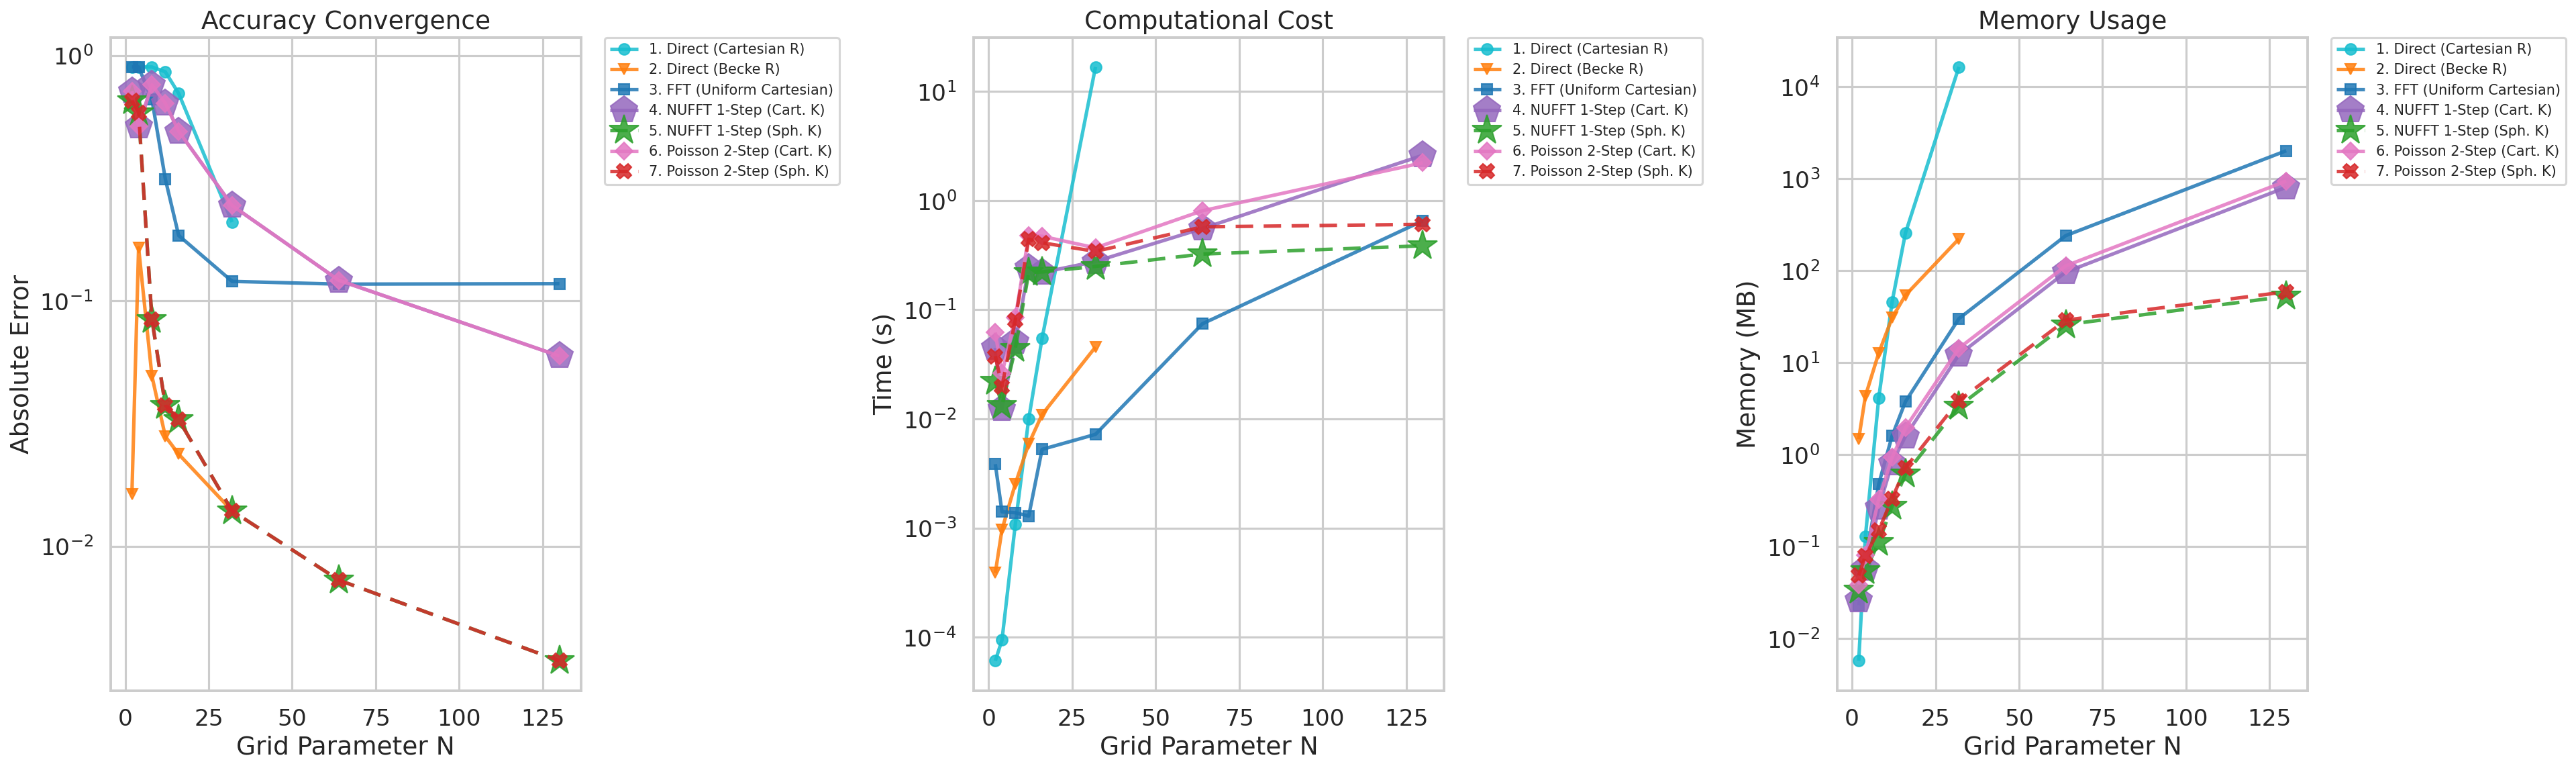
\includegraphics[width=\textwidth]{eri_benchmark.png}
    \caption{Benchmark results for seven ERI computation methods. \textbf{Left:} Absolute error versus grid parameter $N$ (log scale). \textbf{Centre:} Wall-clock computation time (log scale). \textbf{Right:} Peak memory usage (log scale). Methods: (1)~Direct Cartesian, (2)~Direct Becke, (3)~FFT Uniform, (4)~NUFFT 1-step Cartesian $k$, (5)~NUFFT 1-step Spherical $k$, (6)~Poisson 2-step Cartesian $k$, (7)~Poisson 2-step Spherical $k$.}
    \label{fig:benchmark}
\end{figure}

\subsection{Accuracy Convergence}

The left panel of \cref{fig:benchmark} reveals markedly different convergence behaviours:

\paragraph{Direct methods (1--2).} The direct Cartesian method (Method 1) converges slowly, with the error plateauing near $10^{-1}$ even at $N = 32$. This is because the uniform grid poorly resolves the cusp-like density near the nuclei, and the $1/r$ singularity in the Coulomb kernel introduces discretisation artifacts. The direct Becke method (Method 2) converges significantly faster because the atom-centred grid concentrates points where the density is largest. However, both methods share $\mathcal{O}(N^2)$ complexity in the number of grid points, limiting their practical utility.

\paragraph{Uniform FFT (3).} The FFT Poisson solver shows moderate convergence, reaching errors around $10^{-1}$ at large $N$. Its accuracy is fundamentally limited by the uniform grid: the Nyquist frequency $k_{\max} = \pi/\Delta x$ grows only linearly with $N$, and the grid cannot adapt to the non-uniform density distribution. The FFT does benefit from excellent computational scaling, however.

\paragraph{NUFFT one-step methods (4--5).} Both Cartesian and spherical $k$-grid variants benefit from the Becke grid in real space, giving them better resolution near the nuclei. The spherical $k$-grid variant (Method 5, dashed green) converges more smoothly than the Cartesian $k$-grid variant (Method 4) because the spherical quadrature is naturally suited to the isotropic Coulomb kernel, and the $k^2$ cancellation avoids singularity issues. At $N = 64$, Method 5 reaches errors near $10^{-2}$.

\paragraph{Poisson two-step methods (6--7).} The two-step Poisson solver with a spherical $k$-grid (Method 7, dashed red) achieves the best convergence of all methods, reaching errors below $10^{-3}$ at moderate grid sizes and continuing to improve. This superiority arises because the two-step approach constructs a smooth real-space potential $V^{(g)}(\mathbf{r})$ before performing the final integration, which is more amenable to accurate numerical quadrature than the oscillatory $k$-space integrand in the one-step approach. The Cartesian $k$-grid variant (Method 6) also converges well but is hampered by the singularity at $\mathbf{k} = \mathbf{0}$.

\subsection{Computational Cost}

The centre panel of \cref{fig:benchmark} shows wall-clock times on a logarithmic scale.

The direct methods exhibit the steepest scaling, with times reaching nearly one second at $N = 32$ due to $\mathcal{O}(N^6)$ operations for the Cartesian grid. The FFT method scales as $\mathcal{O}(N^3 \log N)$ and is the fastest at small $N$, benefiting from highly optimised FFTW-based implementations. However, it requires $N^3$ grid points, so the absolute cost grows rapidly.

The NUFFT methods (4--7) occupy an intermediate regime. Their cost is dominated by the type-3 NUFFT, which scales as $\mathcal{O}((M + N_k)\log(M + N_k))$ where $M$ is the number of real-space points and $N_k$ the number of $k$-space points. The spherical $k$-grid variants (5, 7) use fewer $k$-points than their Cartesian counterparts because the Lebedev grid is more compact than a Cartesian cube in $k$-space, giving them a consistent speed advantage. At large $N$, all NUFFT methods maintain sub-second runtimes.

\subsection{Memory Usage}

The right panel shows peak memory consumption. Direct methods are memory-intensive because they construct the full $N \times N$ distance matrix. The FFT method uses moderate memory for the 3D grid and its transform. The NUFFT methods are the most memory-efficient of the spectral approaches, since they avoid storing dense matrices and operate on sparse, non-uniform point sets. Methods using spherical $k$-grids consistently use less memory than those with Cartesian $k$-grids because the spherical grid requires far fewer points to achieve comparable angular resolution.


%==========================================================================
\section{Discussion}
\label{sec:discussion}
%==========================================================================

\subsection{Why the Poisson Two-Step Method Excels}

The superior convergence of Method 7 (Poisson two-step with spherical $k$-grid) can be understood from several mathematical perspectives.

First, the two-step formulation separates the forward transform, kernel application, and inverse transform into distinct stages. This means the NUFFT approximation error enters twice but affects different quantities: the forward transform approximates $\widetilde{G}(\mathbf{k})$ and the inverse transform reconstructs $V^{(g)}(\mathbf{r})$. Because $V^{(g)}(\mathbf{r})$ is a smooth Coulomb potential (no cusps or singularities away from the nuclei), the inverse NUFFT achieves high accuracy, and the final real-space integration on the Becke grid is exact to high order.

Second, the spherical $k$-grid exploits the isotropy of the Coulomb kernel. The $4\pi/k^2$ factor depends only on $|\mathbf{k}|$, so a grid with Gauss--Legendre points in the radial direction achieves exponential convergence for smooth radial integrands. In contrast, a Cartesian $k$-grid wastes points in the corners of the cube where $|\mathbf{k}|$ is large, and the integrand is negligible.

Third, the analytical cancellation of $k^2$ between the Jacobian and the Coulomb kernel (\cref{eq:sph_weights,eq:coulomb_ft}) means the effective integrand in $k$-space is $4\pi\,|\widetilde{G}(\mathbf{k})|^2$ weighted by the base quadrature weights, without any singular factor. This makes the quadrature inherently well-conditioned.

\subsection{Limitations of the Direct and FFT Methods}

The direct methods, while conceptually simple, suffer from two compounding issues. The $\mathcal{O}(N^2)$ pairwise summation is inherently expensive, and the discretisation of the $1/r$ singularity introduces systematic errors that diminish slowly with grid refinement. The self-interaction exclusion (setting the distance matrix diagonal to infinity) is a necessary but imperfect remedy.

The uniform FFT method is limited by its inability to adapt to the molecular geometry. All points of the density profile, including the near-nuclear cusps, must be resolved by the same uniform spacing. This results in either insufficient resolution (if $N$ is small) or excessive memory and compute (if $N$ is large enough to resolve the cusps).

\subsection{Cartesian versus Spherical $k$-Space Grids}

A consistent finding across both the one-step and two-step methods is the superiority of spherical $k$-grids. This can be quantified by comparing the number of grid points required: a Cartesian $k$-grid with $N_k$ points per dimension uses $N_k^3$ total points, whereas the spherical grid uses approximately $N_{\text{rad}} \times N_{\text{ang}}$ points, where $N_{\text{ang}}$ is typically a few hundred (from the Lebedev grid). For the same accuracy, the spherical grid requires one to two orders of magnitude fewer points.

Furthermore, the Cartesian $k$-grid introduces a regularisation problem at $\mathbf{k} = \mathbf{0}$ (the Coulomb singularity), which is handled by setting $K^2 = \infty$ for small values. This ad hoc treatment introduces a systematic bias, whereas the spherical grid avoids the issue entirely.

\subsection{Numerical Stability Considerations}

The NUFFT tolerance parameter $\varepsilon$ plays a critical role. In the one-step method, the entire ERI depends on a single forward NUFFT, so a tight tolerance ($\varepsilon = 10^{-8}$) is required. In the two-step method, the tolerance can be relaxed to $\varepsilon = 10^{-5}$ because errors in the forward and inverse transforms partially cancel when computing the inner product. This tolerance asymmetry is both a practical advantage (faster NUFFT execution) and a theoretical expectation from the variational nature of the energy functional.


%==========================================================================
\section{Conclusion}
\label{sec:conclusion}
%==========================================================================

This study benchmarked seven numerical methods for computing electron repulsion integrals on the H$_2$ molecule. Our principal findings are as follows:

\begin{enumerate}
    \item The \textbf{Poisson two-step NUFFT with spherical $k$-space quadrature} (Method 7) achieves the best accuracy--efficiency trade-off, converging below $10^{-3}$ absolute error with moderate grid sizes and competitive wall-clock times. The analytical cancellation of the $k^2$ Jacobian with the Coulomb kernel singularity is the key mathematical insight enabling this performance.

    \item \textbf{Becke molecular grids} in real space consistently outperform uniform Cartesian grids across all methods that use them, confirming that adaptive, atom-centred quadrature is essential for molecular integrals.

    \item \textbf{Spherical $k$-grids} outperform Cartesian $k$-grids in both accuracy and efficiency, due to better alignment with the isotropic Coulomb kernel and natural singularity cancellation.

    \item \textbf{Direct summation} methods, while useful as baselines, are impractical beyond small grid sizes due to $\mathcal{O}(N^2)$ scaling.

    \item The \textbf{uniform FFT} serves as a middle ground but is fundamentally limited by its inability to adapt to non-uniform density distributions.
\end{enumerate}


\bibliographystyle{unsrtnat}
\bibliography{references}

\end{document}
